\section{Testarten}
\label{sec:TestUndNorm}
%Welche Testarten gibt es?
%Welche sind sinnvoll bei unserer Schaltung?
%Norme vellicht bi dr Uswertig ihne? oder bi de teschts?

Im EMV-Unterricht haben wir gelernt, dass es fünf sehr wichtige Normstörungen gibt, auf welche wir die Schaltung testen könnten. Da wären ESD (Electrostatic Discharge bzw), Burst, Surge, HF-Störfelder und die gestrahlte Emission. Im nachfolgenden werden die einzelnen Normstörungen kurz erläutert und die Wahl der gewählten Normstörungen begründet.
\subsection{ESD}

\subsection{Burst}
%Was ist Burst?
Der Burst ist eine HF-Störung, welche Leitungsgebunden ist. HF-Störungen können häufig durch Schaltvorgänge (z.B. prellen eines Tasters, einstecken eines Adapters...) in das System eingekoppelt werden. Dieses Prüf- und Messverfahren zur Prüfung der Störfestigkeit gegen schnelle transiente elektrische Störgrössen (Burst) unterliegt der Norm EN 61000-4-4.\\[0.25cm]
%Was wird beim Test gemacht?
Über eine kapazitive Koppelzange werden schnelle transiente Störgrössen (Bursts) auf Leitungen gegeben. Diese Bursts verfügen mit bis zu 400MHz über ein weites Störspektrum und können Amplituden bis zu einigen kV haben.\\

\begin{minipage}[b][6cm][t]{1\textwidth}
\centering
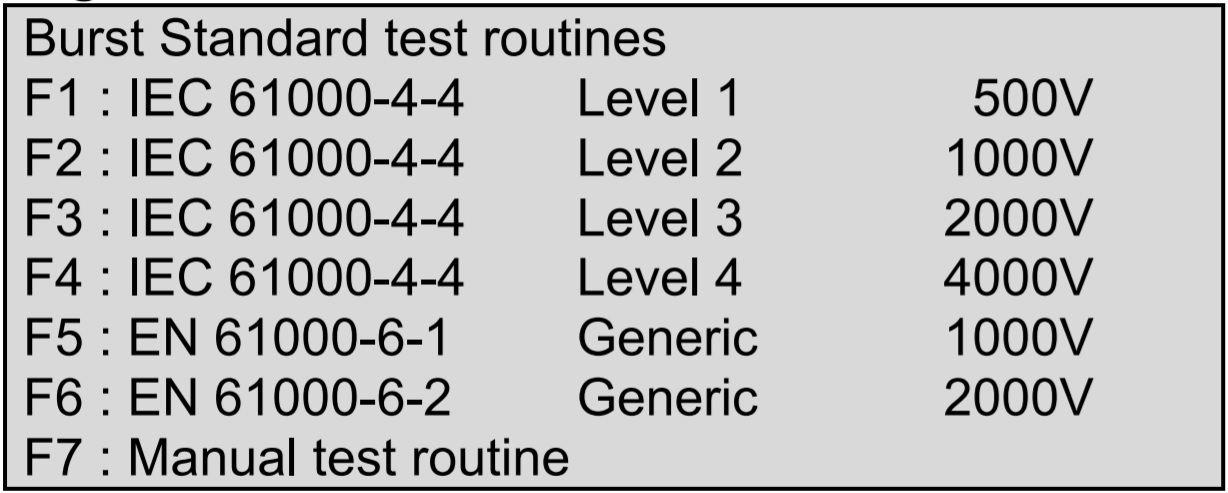
\includegraphics[angle=0,width=0.75\textwidth]{graphics/BurstProgramm.jpg}
\captionof{figure}{Die Burst-Programme für die verschiedenen Testlevel.}
\label{fig:BurstProgramm}
\end{minipage}

Abbildung \ref{fig:BurstProgramm} zeigt die verschiedenen Burst Standart Test Routinen an. Deutlich zu erkennen ist, dass es verschiedene Level mit verschiedenen Amplituden gibt.\\

\subsection{Surge}
Die Surge-Impulse werden bei EMV-Tests verwendet um die Verträglichkeit gegen Stossspannungen (Impulse) zu testen. Solche Stossspannungen können bei Blitzeinschlägen oder Schaltvorgängen in der Versorgungsleitung auftreten. Dieses Prüf- und Messverfahren zur Prüfung der Störfestigkeit gegen Stossspannungen (Surge) unterliegt der Norm EN 61000-4-5.\\[0.25cm]
Über ein Surge-Generator werden Impulse mit hoher Spannung auf eine Leitung gegeben. Dabei ist wichtig, dass ein Entkopplungsnetzwerk verwendet wird. Dies verhindert, dass die Impulse statt auf das Testobjekt auf das Stromnetz gegeben werden.\\

\begin{minipage}[b][6cm][t]{1\textwidth}
\centering
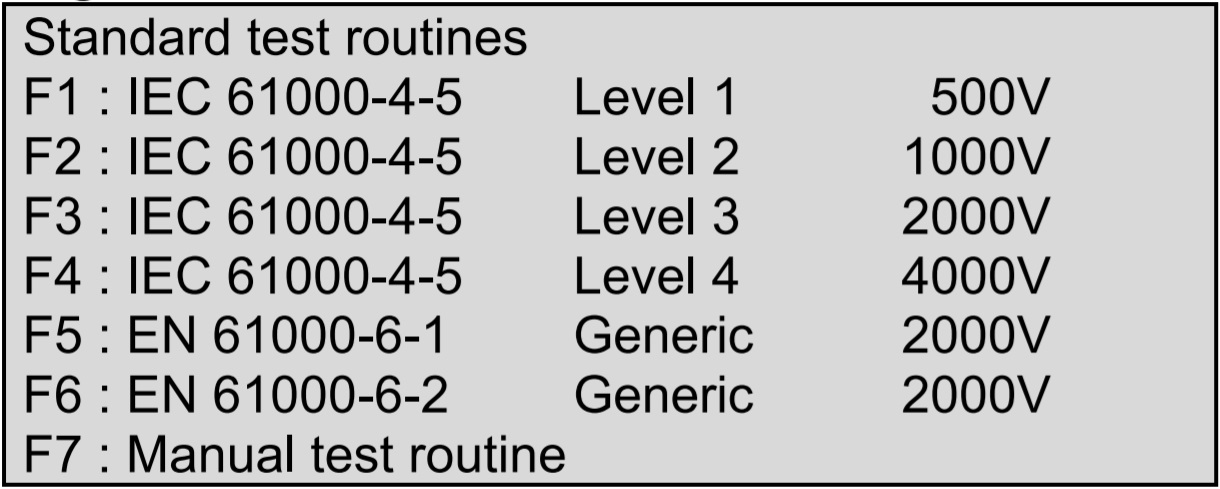
\includegraphics[angle=0,width=0.75\textwidth]{graphics/SurgeProgramm.jpg}
\captionof{figure}{Die Surge-Programme für die verschiedenen Testlevel.}
\label{fig:SurgeProgramm}
\end{minipage}

Abbildung \ref{fig:SurgeProgramm} zeigt die verschiedenen Surge Standart Test Routinen an. Auch hier ist deutlich zu erkennen, dass es wiederum vier verschiedene Level gibt, mit verschiedenen Amplituden, welche der Norm entsprechen.\\

\subsection{HF-Störfelder}

\subsection{Gestrahlte Emission}

\subsection{Auswahl der EMV-Tests und Kriterien}
Verschiedene Systeme werden in den verschiedensten Gebieten eingesetzt, weshalb es auch immer wichtig ist zu spezifizieren welche EMV-Tests sinnvoll sind und welche Kriterien diese erfüllen sollen.\\[0.25cm]
Die gewählte Schaltung soll stellvertretend für eine in einem System integrierte Schaltung sein. Erwähntes System hat eine hohe Bauteildichte und wird mit einem Gehäuse geschützt, weshalb ein direkter Zugriff auf die Schaltung während des Betriebs nicht erfolgen kann. Aus diesem Grund wird kein ESD-Test durchgeführt. Ausserdem sind die EMV-Tests für Störfelder und gestrahlte Emission ebenso weniger interessant. Jedoch sind die Burst- und Surge-Tests interessant, da der Strom eines Motors angehängt wird und dieser allenfalls über längere Leitungen verbunden wird.\newline
Die Erfüllungskriterien der EMV-Tests können in Funktionslevel eingestuft werden. Bei Funktionslevel A muss das Gerät auch während des Tests weiterhin wie beabsichtigt funktionieren. Bei Funktionslevel B muss das Gerät nach dem Test weiterhin wie beabsichtigt funktionieren. Bei Funktionslevel C ist ein vorübergehender Funktionsverlust zulässig, vorausgesetzt, das System kann seine Funktionalität selbst wiederherstellen.\newline
Da Strommessungen oft gemittelt werden, ist ein kurzer Ausfall annehmbar, weshalb ein Funktionslevel B angestrebt wird.\\[0.25cm]
Die Schaltung wird somit auf die Normstörungen Burst und Surge getestet und ein Funktionslevel B wird für alle Tests angestrebt.\\

Nun wurde die Schaltung vorgestellt und die EMV-Tests ausgewählt. Bevor es zu den Testprotokollen kommt, muss im nächsten Kapitel auf die verwendeten Schutzelemente eingegangen werden.